\chapter{论文相关基础知识与技术}
本章首先说明智能体的基本概念;然后介绍当前热门的智能体架构-BDI(Belief-Desire-Intention)智能体架构,然后介绍BDI智能体信念、动作计划和目标的规范表示,然后介绍一种表示BDI智能体意图的数据结构-目标计划树(Goal-Plan Tree,GPT),最后基于此对意图进展问题进行规范定义。

\section{智能体系统与BDI智能体架构}\label{background}
\subsection{智能体系统}
智能体在现代社会有着广泛的应用,然而不同领域对智能体的定义也不尽相同。本文遵循\cite{DBLP:journals/ker/WooldridgeJ95}中对智能体的定义,智能体是一种处于一定环境下能够自主、智能地完成其他个体指派任务的计算机系统,其遵循感知--执行动作的周期性运作流程。其最大的特点是自主性、社会性、反应性以及主动性。
\begin{itemize}
  \item 自主性:自主性是智能体最核心的特性,其指的是指智能体能够自主地进行一系列行为,比如判断、计算和做出动作,以实现人们指定的目标。这种自主的表现都是基于内部状态和智能体的行为能力,内部状态是智能体对自身所处状态的理解,即智能体认为它是怎么样的、处于什么状态、目的是什么。而行为能力是指智能体根据内部状态进行自主的判断,能做出一些具体的行为来影响其周围的环境或改变自身的处境。自主性使得智能体决策以及行为由其自身控制,而非由其他个体操纵。
  \item 社会性:在多智能体系统(Multi-Agent Systems,MAS)中,智能体之间会进行交互,比如合作完成任务,或者在比赛中竞争,表现出社会性。在社会性的交互中,信息交流是不可或缺的,智能体须通过交流的语言、协议、信息本身对信息进行发送或接收处理,同时智能体根据交互的信息对系统中其它智能体建立认知模型,以更好地使智能体共同完成一些特定目标。
   \item 反应性:智能体能够感知到环境中的事件或发生的一些变化并及时的做出一些决策或行为来进行响应,以便实现指定目标。这种能力使得智能体在完成指定目标的过程中能够更加灵活地应对环境中的变化。
   \item 主动性:智能体的行为是以目标为导向的,其能够主动采取行动来实现给定的目标,而不是完全被动地等待,拒绝尝试对实现目标有帮助的行为。
\end{itemize}

\subsection{BDI智能体架构}
实现智能体的方式有多种,不同的实现方式对应了不同的智能体架构。目前已有多种智能体架构被提出,例如慎思型智能体架构(Deliberative agent Architecture),反应型智能体架构(Reactive Agent Architecture)以及混合型智能体架构(Hybird Agent Architecture)。本文的关注重点为BDI智能体架构(Belief-Desire-Intention Agent Architecture)。BDI智能体架构是当前热门且成熟的智能体架构,其起源于Bratman的关于实践推理(Practical Reasoning)的哲学理论\cite{bratman1987intention}。为了对人类的心理状态进行模拟,BDI智能体架构明确地将智能体的内部状态以一组特殊的数据结构表示,即信念、欲望和意图。基于BDI智能体架构的智能体被称为BDI智能体。
% Bielief
在BDI智能体中,信念表示的是BDI智能体所相信的事件或状态,例如在某个位置、目前的速度或当前的外部环境情况等等,然而信念并不一定是事实,仅仅代表BDI智能体的认知,BDI智能体会根据自身对环境的感知或自身做出的行为改变环境进而改变信念,或是将信念作为参考做出一系列的判断或行为。
% Desire
愿望指的是BDI智能体想要实现的环境环境状态。欲望可以是没有具体实现方案去实现的,甚至不可实现的,也可被视为一些未实例化的想法,而并没有确定去如何做,做什么。此外当智能体同时有多个意图时,由于没有实例化或决定实现这些意图,意图与意图之间可以有冲突,例如BDI智能体可以同时拥有进行休眠充电和打扫卫生这两个愿望,即使这二者是相互冲突的。
% 目标
目标(Goal)指的是一组智能体确定要去实现的愿望,也就是说一个目标对应于一个实例化的愿望,即智能体知道要实现什么并且承诺尝试去实现。目标的种类主要有两种:实现型目标(Achievement Goal)和维持型目标(Maintenance Goal)。
% acheivement goal
实现型目标表示智能体想要达到的世界状态,一旦该状态达成,其相应的实现型目标就会被丢弃。例如,智能体有一个去超市电池的实现型目标,一旦购买成功,无需重复购买,智能体便会丢弃该目标。

% Maintenance goal
维持型目标要求智能体在一段时间内(或者一直)维持某一世界状态。和实现型目标不同的是,维持型目标被满足后并不会被丢弃,而是仍然存储于智能体的内部。智能体会对维持型目标持续监控,直到其过期。在此期间一旦维持型目标被破坏,智能体便会尝试修复该目标状态,这种情况下智能体对待维持型目标的方式是被动的,即等到维持型目标被破坏再尝试修复,以被动方式应用的维持型目标被称为被动维持型目标(Reactive Maintenance Goal)。此外,智能体还可以在维持型目标被破坏之前对其是否在将来会被破坏进行预测评估,如果预计在将来的某个时刻维持型目标会被破坏,智能体还可以采取主动措施防止其被破坏,以该种主动方式应用的维持型目标被称为主动维持型目标(Proactive Maintenance Goal)。在本文中,维持型目标是一个重要的研究内容;后文将对维持型目标的相关调度算法进行细致阐述并进行性能评估。

%Intention
意图(Intention)为实例化的计划,用以实现某个目标。而计划的内部--计划体由动作和子目标组成。动作的执行可以直接影响外部环境,而子目标可由其他子计划实现。 当智能体承诺要实现某个目标时,便需要执行一个具体的计划来实现对应的目标。一个目标可由多个不同的计划来实现,智能体只要选择其中一个计划执行即可,即智能体会从该目标对应的可选计划中根据具体实际情况,判断并选择一个计划,通过执行选中的计划来完成相应目标,这种多个计划的设计也使得智能体可以灵活应对不同的环境。由于计划体也可以包含子目标,在运行过程中,会递归性地选出并执行多个计划,从具体实现的角度来说,每个意图都是一个栈,里面存储的就是部分实例化的计划,意图的执行也就对应于执行栈中一系列的计划。

% Practical Reasoning
在BDI智能体架构中,智能体进行决策的流程被称为实践推理(Practical Reasoning)。和纯粹的逻辑推理或理论推理不同,实践推理是以行为为导向的,即决定做什么以及如何去做。例如,假设Alice是Bob女儿,Carl是Alice的儿子。则基于逻辑推理可知Carl是Bob的孙子,该种推理方式仅仅依赖智能体的信念以及一些逻辑规则;相较于此,决定该乘坐何种交通工具上学的决策过程则是实践推理的范畴,因为其包含对“如何做”的考虑,是以行为为导向的推理。

% deliberation and means-ends reasoning
Bratman\cite{bratman1987intention}认为实践推理可被看做智能体基于其内部状态,(即信念、愿望等),在多个相互冲突的选择中进行权衡考量,做出合理的决策的过程。
%
具体地,实践推理主要有两步构成:慎思(Deliberation)和手段推理(Means-Ends Reasoning)。
%
在第一步慎思过程中,智能体考虑要去实现哪个目标,即生成目标对应的意图,意味着智能体决定要去尝试实现该目标。
%
而在第二步手段推理过程中,智能体考虑如何实现某个目标,即对于上一步确定要实现的目标,决定执行哪一个计划去实现。
% example
例如,假设智能体现有两个愿望:前往超市购买食物和在家打扫卫生;在经历慎思过程后,智能体决定前往超市。而前往超市有两种途径:走路前往和开车前往;智能体决定走路前往还是开车前往的过程即为手段推理。

\subsubsection{BDI智能体程序的执行}
为了实现BDI智能体程序,Bordini\cite{bordini2007programming}描述了BDI智能体运行的控制流,其具体流程如图\ref{fig:deliberation}。
\begin{figure*}[htb]
\centering
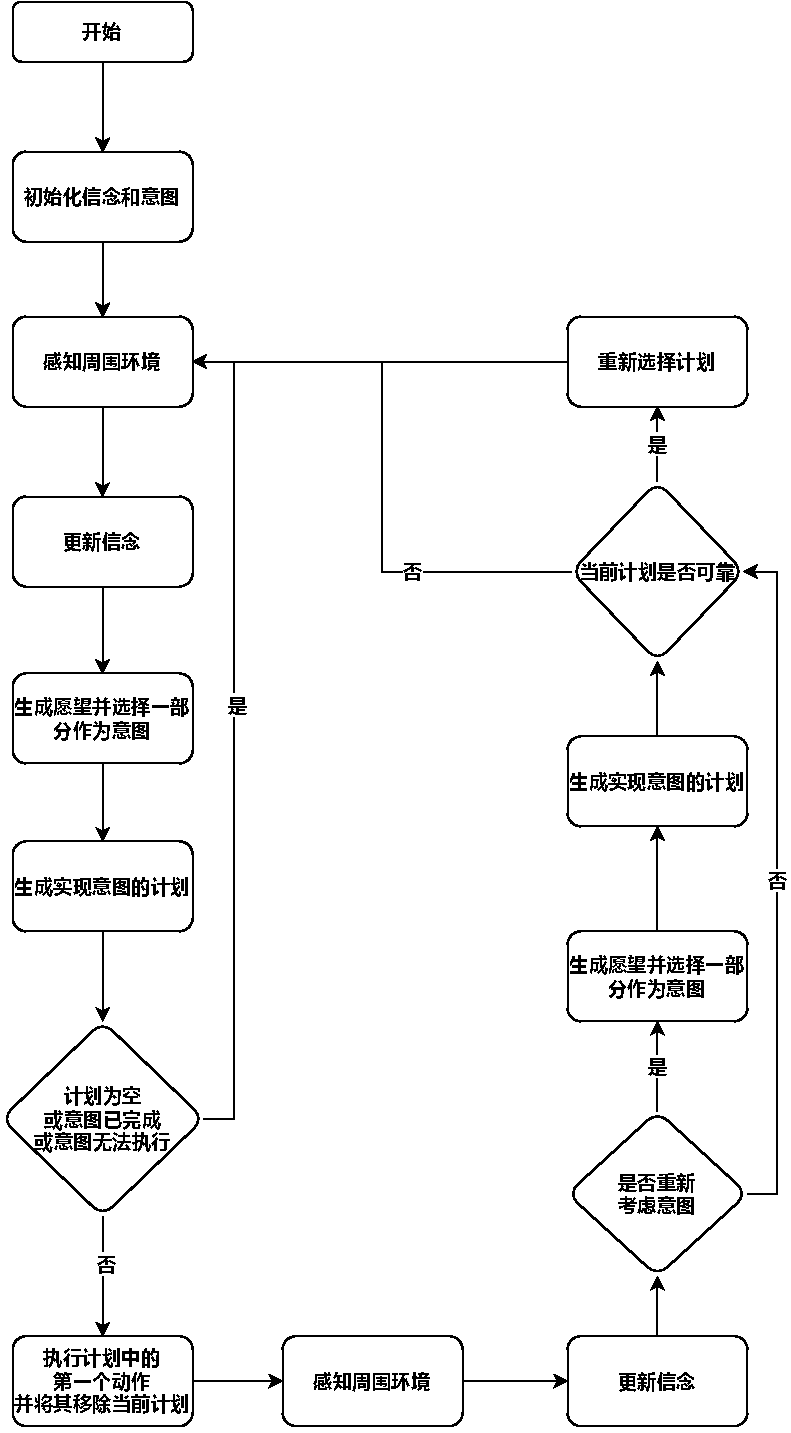
\includegraphics[scale=0.6]{./figs/deliberation_cycle}
\bicaption{BDI智能体的执行流程}{Overall control loop of BDI agent}
\label{fig:deliberation}
\end{figure*}

在执行动作之前,智能体首先对周围环境进行感知,并对自身的信念进行更新,然后智能体根据更新后的信念以及当前的意图得到新的愿望,并选择部分愿望生成对应的意图,最后选择计划以实现意图。理想情况下,在具体执行时智能体依次执行计划中的每一个动作直至计划计划中的所有动作都执行成功。然而,由于环境是多变而不确定的,智能体在执行完一个动作之后需要对环境进行感知并更新其信念,并决定是否要重新考虑意图。由于重新考虑意图需要额外的计算开销,通常情况下智能体不会频繁地进行重新考虑的操作,而是当确定重新考虑会对当前的意图造成改变时进行该操作。即如果重新考虑不会对当前意图造成影响,那么智能体无须在执行过程中浪费计算资源而是直接执行当前的意图。最后,无论是否重新考虑意图,智能体判断当前的计划是否依然合理或是否值得继续执行。如果当前计划被判断为不适合继续执行,智能体将重新进行计划选择。

\section{BDI智能体的表示与问题定义}
\subsection{信念、计划以及动作的规范表示}
本节主要介绍BDI智能体信念、动作、计划以及目标这四个基本元素的规范表示,在后续的章节中根据问题场景不同将会介绍到BDI智能体其他属性的规范表示。
\paragraph{信念}
信念为智能体对环境及其自身的认知,一个信念以一个实例化的一阶谓词公式表示:
$$P(t_1, \ldots,t_n)$$
其中$P$为谓词,$t_1, \ldots,t_n$为实例化的个体变元。例如有一谓词公式$Battery(\beta, x)$表示智能体$\beta$当前的电量为$x$,其中$\beta$为一变量指代某一个智能体,$x$为一常数变量,则$Battery(Alice, 60)$这条信念表示智能体$Alice$当前的电量为$60$。
\paragraph{动作}
动作是智能体可以执行的最小单元,其可以直接对环境造成影响。一个动作以一个三元组表示:
$$<A,C_{pre},C_{post}>$$
其中$A$为该动作的名称,$C_{pre}$和$C_{post}$分别对应该动作的前置条件和后置条件。与信念的表示相同,每个条件(前置条件和后置条件)以一阶谓词公式表示。
\paragraph{计划}
每个计划P以$G:\emptyset \gets \alpha_1; \dots;\alpha_n$的形式表示,其中G为一个目标,$\emptyset$是一组命题公式,为该计划的前置条件,只有当$\emptyset$为真时,P才能被执行。最后,$\alpha_1; \dots;\alpha_n$为计划中的一些列执行步骤,计划的执行对于依次执行这些执行步骤。每个执行步骤或为可以直接改变环境的动作或为子目标,而子目标可其对应的子计划实现。
\paragraph{目标}
$$<G_a,C_g,Pls>$$
其中$G_a$为该目标的名称,$C_g$为目标条件,即一组智能体想要达到的条件。每个目标都与一组用于实现该目标的计划$Pls=\{P_1,\dots,P_n\}$相关联。一旦目标条件被达成,智能体便会抛弃该实现型目标。

\subsection{目标计划树}
% ref
Thangarajah等人\cite{DBLP:journals/jar/ThangarajahP11,DBLP:conf/ijcai/ThangarajahPW03,DBLP:conf/ijcai/ThangarajahPW03,DBLP:conf/ecai/ThangarajahWPF02}提出目标计划树(Goal-Plan Tree)的数据结构来表示BDI智能体目标及计划之间的关系。在此基础上,Yao等人\cite{DBLP:conf/atal/YaoSL16}提出了对目标计划树的拓展,增加了对动作的表示,定义了包含多种可能后置条件的易错动作和有执行时间的持续型动作,并提出了一种基于控制变量合成随机目标计划树的方法\cite{patent0}作为基准测试平台对不同的意图调度算法进行评估比较。目标的定义也被拓展为含有截止时间和期望完成时间。考虑到目标计划树的表达能力,本文将使用Yao等人提出的拓展目标计划树来表示智能体的意图。

% GPT
目标计划树的根节点为顶层目标节点,即智能体想要达到的最终目的;其孩子节点为一个或多个计划节点。每个计划节点的孩子节点为一系列执行步骤(动作或子目标);而子目标又有其对应的计划节点,如此便构成了树形结构,其展现了所有实现顶层目标的途径。此外,为了实现某个目标,智能体只需要选择一个计划执行即可,因此计划节点也被视为“OR”节点;而为了完整执行一个计划,智能体需要依次成功执行其对应的所有执行步骤,因此计划节点的孩子节点被视为“AND”节点。

图\ref{fig:gpt}展示了火星探测器领域下的一个简单目标计划树模型,其中环境为$h*w$的网格。火星探测器智能体可以通过执行动作在不同的方格中移动。其顶层目标$G0$表示将智能体移动到$(a,b)$位置。有五个不同的计划可用于实现$G0$,不同的计划可应用于不同的环境状态下。如果智能体当前位置位于$(x,y)$且$y < b$,则计划$P0$可用于实现$G0$。P0由两个步骤组成,一个是可直接执行的动作$A0$,执行$A0$可以使智能体向上移动一个单位,第二个是子目标$G0$,$G0$为递归目标(即该子目标实际与顶层目标相同)。$A0$的前置条件为智能体不在网格的上边界(在上边界执行该动作会使得智能体超出边界范围),而其后置条件则为将智能体位置至于$(x,y+1)$。另外,该目标计划树示例将用于后续章节的实验部分。
\begin{figure*}[htb]
\centering
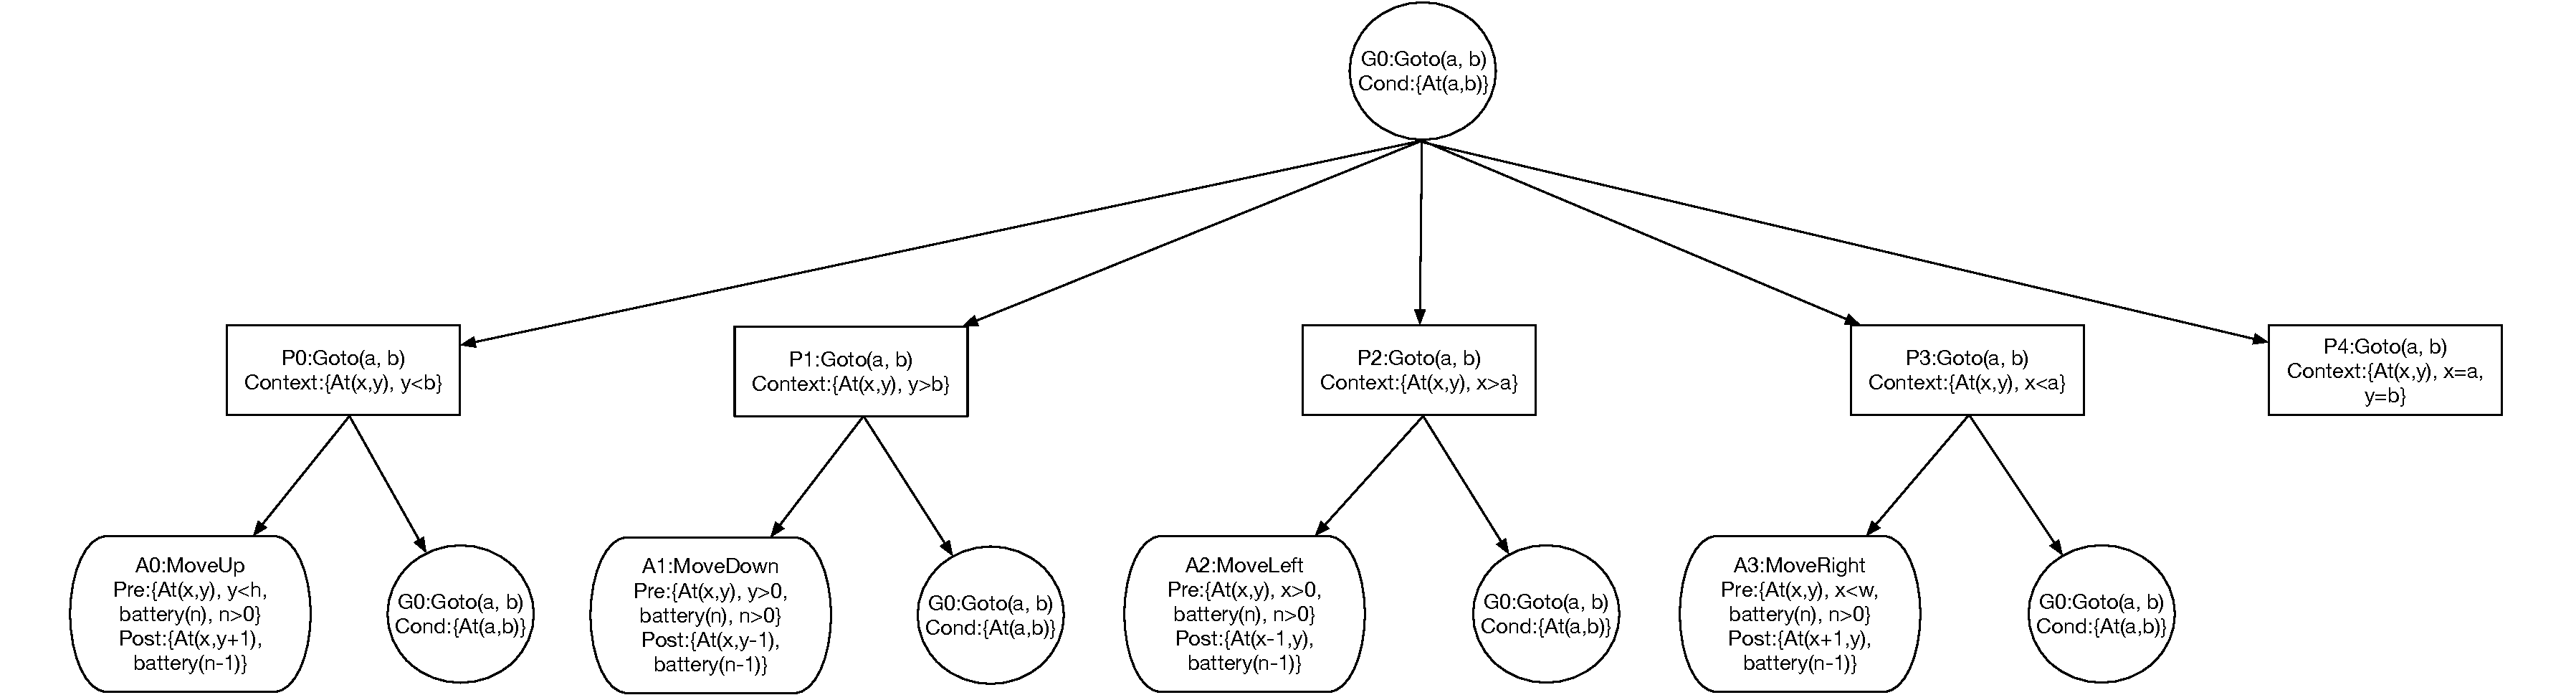
\includegraphics[scale=0.23]{./figs/MarsRover_GPT}
\bicaption{目标计划树例子}{Example goal-plan tree}
\label{fig:gpt}
\end{figure*}

% Benefits of GPT representation
目标计划树直观地展现了智能体目标、计划和动作之间的关系。除此以外,目标计划树还可用于记录实现目标或执行计划和动作所需的前置条件(Precondition)以及执行的结果,后置条件(Postcondition)。计划的前置条件指的是执行计划前需要满足的条件,如果前置条件不满足,则计划无法执行(动作的前置条件同理)。后置条件指的是执行动作之后的结果,对智能体所处环境造成的影响。最后,目标计划树还可以用于刻画智能体在某个环境下实现特定目标时的健壮性,Thangarajah等人基于目标计划树提出Coverage和Overlap的概念\cite{DBLP:conf/aamas/ThangarajahSP12}以刻画智能体程序的健壮性。其中Coverage表示一个意图当前的目标或子目标至少有一个计划可执行情况下可能的环境状态占比;而Overlap则表示一个目标有多个(大于一个)可执行计划的情况下可能的环境状态占比。

\subsection{意图进展问题}
上一小节介绍了目标计划树的概念,本章节基于目标计划树,对BDI智能体意图进展问题进行规范定义。

BDI智能体通常有多个计划用以实现某一个目标,不同的计划根据其前置条件不同适用于不同的环境场景,前置条件满足的计划被称为可应用计划(Applicable Plan)。
% plan selection
当同时有多个可应用计划是,智能体需要考虑选择哪一个计划用以实现相应目标,该问题被称为计划选择问题(Plan Selection Problem)。计划选择会影响到并发执行的其他目标,因为不同的计划有着不同的后置条件,这些后置条件可能会影响其他目标下计划或动作的前置条件。这种影响可能是负面的,例如一个计划执行之后使得其他目标下的某些计划的前置条件失效,也有可能是正面的,例如一个目标下的某些计划的前置条件在初始时是不满足的,当执行其他目标下的计划之后使得其前置条件满足。

% intention selection
另一方面,当智能体有多个意图时,下一步该执行哪个意图的问题被称为意图选择问题(Intention Selction Problem)。意图选择问题同样也会影响目标的实现,不合理的意图选择可能会造成各个意图中的前置条件相互破坏,导致无法实现任何一个目标(单个目标本身可以顺利实现),而合理的意图选择则可以使得多个意图产生协同效应,相互促进执行。

% IPP
意图进展问题(Intention Progression Problem)为上述两问题的结合,即同时考虑计划选择问题和意图选择问题。意图进展问题是本文所研究的问题的基础。为了规范并一般化地表示意图进展问题,本文基于目标计划树对意图进展问题进行定义。一个意图的进展实际对应于一个目标计划树中一条从根节点到一个叶子结点的路径。目标计划树中的任何一条从根节点至叶子节点的路径都对应于实现其顶层目标的一种方式。每一条路径都包含一系列的计划、动作和子目标,如果他们都被成功执行,即可实现顶层目标。如此,智能体的执行过程可看作多个目标计划树执行路径的相互交错,即对应于意图进展的并发执行。

%
在不同场景下对智能体性能的评估标准可能不同,例如,有时智能体完成目标的数量越多越好,而有时公平性更重要,多个目标的完成时间越接近越好。为了在社会仿真模拟场景下提供一个一般化的意图调度方法,本文假设对某一场景下的智能体有一价值函数$f_{\mu}$,$f_{\mu}$的输入参数为智能体状态信息,并返回一个评估值,代表智能体当前的性能表现。$f_{\mu}$函数可由用户自定义,以应用于不同的问题场景。

% definition
基于上述内容,意图进展问题可被理解为:如何选择多个目标计划树的交错执行路径,使得最终基于$f_{\mu}$获得最大的价值。具体的,给定一组表示智能体意图的目标计划树集合$\{t_1, \dots, t_n\}$,当前环境信息$Env$,智能体的初始状态$S_0$,需要实现的目标集合$G_0$以及当前问题中的价值函数$f_{\mu}$,智能体在每一个运行周期中求解并执行目标选择,计划选择以及意图选择,直到某个最终状态$S$停止运行,要求最终状态$S$使得价值函数$f_{\mu}$的值最大,即智能体从初始状态$s_0$开始进行目标计划树的交错执行,不存在某个最终状态$S^{\prime}$,使得$f_{\mu}(S^{\prime})$的值大于$f_{\mu}(S)$。

% \subsection{对意图进展问题的拓展}
考虑到智能体应用场景的多样性,本文对上述意图进展问题进行拓展作为本文的主要研究问题。本文考虑三类对意图进展问题的拓展:维持型目标下的意图进展问题,norm约束下的意图进展问题以及以LTL为输入的意图进展问题。

\paragraph{维持型目标下的意图进展问题}
考虑到维持型目标通常应用在资源有限的场景中,在该问题定义中,价值函数考虑到了资源消耗。具体地,基于目标计划树模型,维持型目标下的意图进展问题可被定义为:给定一组表示智能体意图的目标计划树$\{t_1, \dots, t_n\}$以及一组表示智能体当前环境状态的条件变量$Env$,在每一个执行周期中返回一个目标计划树$t_i$中的下一个执行步骤使得智能体实现目标所获得的收益最多且消耗的资源量最少。
\paragraph{norm约束下的意图进展问题}
该问题定义对意图进展问题的原始定义进行扩展,加入norm的限制,使得智能体必须同时考虑目标(如何实现目标)以及norm(如何避免违反norm)。具体地,基于目标计划树模型,维持型目标下的意图进展问题可被定义为:给定一组表示智能体意图的目标计划树$\{t_1, \dots, t_n\}$、一组表示当前norm的集合 $N$。以及一组表示智能体当前环境状态的条件变量$Env$,在每一个执行周期中返回一个目标计划树$t_i$中的下一个执行步骤使得智能体实现目标所获得的收益最多且违反norm受到的惩罚最少。
\paragraph{以LTL对象为输入的意图进展问题}
该问题定义加入对LTL表示的目标与norm的考虑。具体地,基于目标计划树模型,以LTL为输入的意图进展问题可被定义为:给定一组表示智能体意图的目标计划树$\{t_1, \dots, t_n\}$,一组智能体需要满足的LTL公式与其对应价值以及一组表示智能体当前环境状态的条件变量$Env$,在每一个执行周期中返回一个目标计划树$t_i$中的下一个执行步骤使得智能体获得的总价值最高。
